\section{Finding Hotspots}

\subsection{Data}
\subsubsection{Why do we use clustering?}
\subsubsection{What data do we cluster?}
\subsubsection{What noise can be expected?}
\begin{frame}
\frametitle{Why do we use clustering?}
	\begin{itemize}
		\item Because ...
	\end{itemize}
\end{frame}	
\begin{frame}
\frametitle{What data do we cluster?}
	\begin{center}
		%Make better example picture with standards from program.
		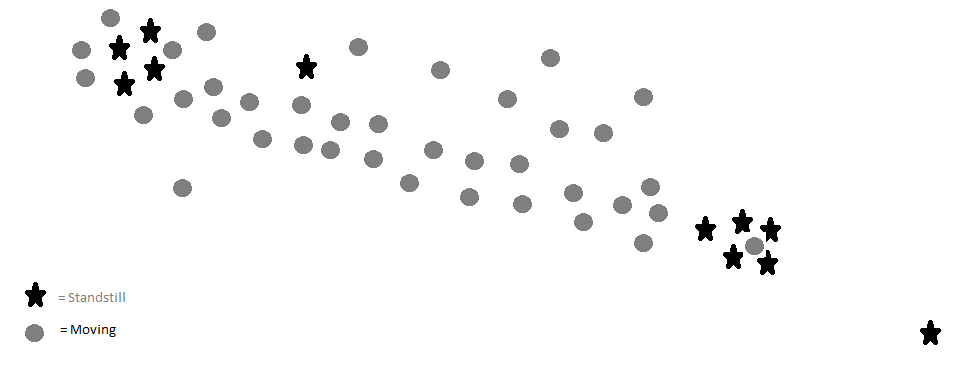
\includegraphics[scale=0.5]{graphics/pointtype-example}
	\end{center}
\end{frame}	
\begin{frame}
\frametitle{What noise can be expected?}
	\begin{center}
		%Make example picture with noise points.
		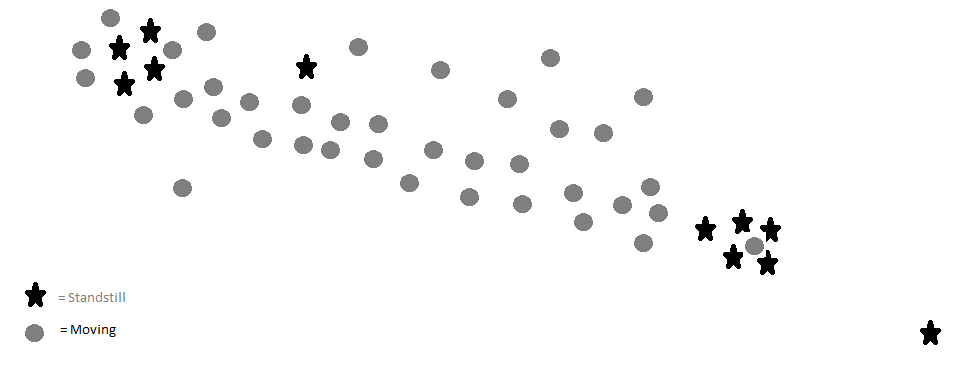
\includegraphics[scale=0.5]{graphics/pointtype-example}
	\end{center}
\end{frame}	


\subsection{Clustering}
%\subsubsection{What is Clustering?}
\subsubsection{Why do we use DBSCAN?} %Partial Clustering? - from presentation notes.
%\begin{frame}
%\frametitle{What is Clustering?}
%	\begin{itemize}
%		\item Because ...
%	\end{itemize}
%\end{frame}	
\begin{frame}
\frametitle{Why do we use DBSCAN?}
	\begin{itemize}
		\item Expected data:
		\begin{itemize}
			\item Partitional - No need for hierarchies.
			\item Exclusive - Separated clusters.
			\item Partial - Need for expected outliers.
			\item Density based - The number of data points is important.
		\end{itemize}
		\item DBSCAN ...
	\end{itemize}
\end{frame}	


\subsection{Convex Hull}
\subsubsection{How does Convex Hull work?}
\subsubsection{Other reduction strategies}
\begin{frame}
\frametitle{How does Convex Hull work?}
	\begin{center}
		%Before/After images of Convex Hull
		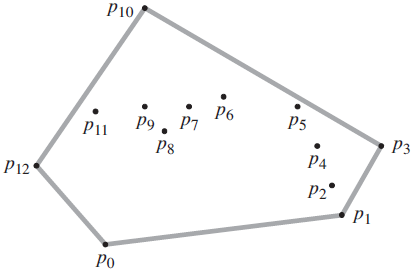
\includegraphics[scale=0.5]{graphics/convexHull-example}
		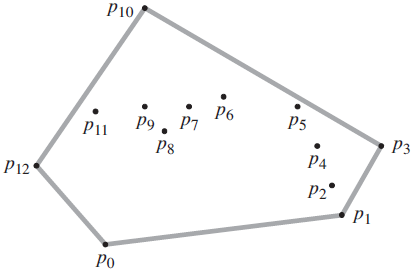
\includegraphics[scale=0.5]{graphics/convexHull-example}
	\end{center}
\end{frame}
\begin{frame}
\frametitle{Other reduction strategies - Square}
\begin{multicols}{2}
	\begin{itemize}
		\item Advantages:
		\begin{itemize}
			\item Property ...
		\end{itemize}
		\item Disadvantages:
		\begin{itemize}
			\item Property ...
		\end{itemize}
	\end{itemize}
\columnbreak
	\begin{center}
		%Images of Convex Hull vs Square
		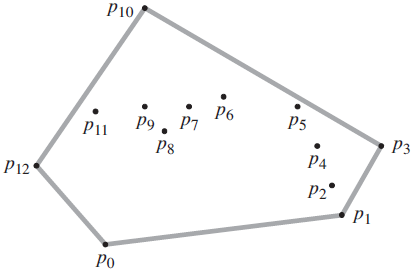
\includegraphics[scale=0.5]{graphics/convexHull-example}\\
		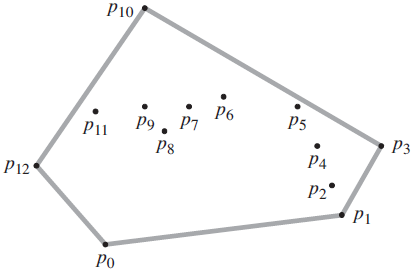
\includegraphics[scale=0.5]{graphics/convexHull-example}
	\end{center}
\end{multicols}
\end{frame}
\begin{frame}
\frametitle{Other reduction strategies - Circle}
\begin{multicols}{2}
	\begin{itemize}
		\item Advantages:
		\begin{itemize}
			\item Property ...
		\end{itemize}
		\item Disadvantages:
		\begin{itemize}
			\item Property ...
		\end{itemize}
	\end{itemize}
\columnbreak
	\begin{center}
		%Images of Convex Hull vs Circle
		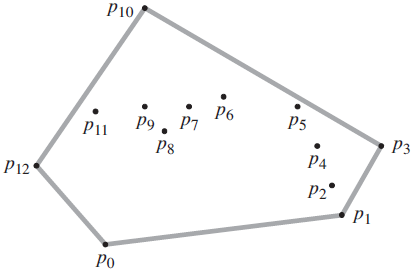
\includegraphics[scale=0.5]{graphics/convexHull-example}\\
		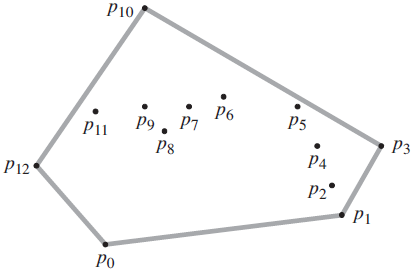
\includegraphics[scale=0.5]{graphics/convexHull-example}
	\end{center}
\end{multicols}
\end{frame}	
\begin{frame}
\frametitle{Other reduction strategies - Polygon}
\begin{multicols}{2}
	\begin{itemize}
		\item Advantages:
		\begin{itemize}
			\item Property ...
		\end{itemize}
		\item Disadvantages:
		\begin{itemize}
			\item Property ...
		\end{itemize}
	\end{itemize}
\columnbreak
	\begin{center}
		%Images of Convex Hull vs Polygon
		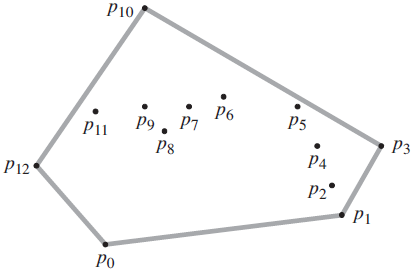
\includegraphics[scale=0.5]{graphics/convexHull-example}\\
		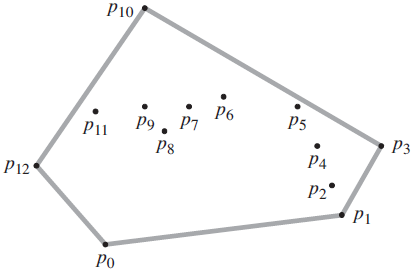
\includegraphics[scale=0.5]{graphics/convexHull-example}
	\end{center}
\end{multicols}
\end{frame}	